% !TEX TS-program = pdflatex
% !TEX encoding = UTF-8 Unicode

% This is a simple template for a LaTeX document using the "article" class.
% See "book", "report", "letter" for other types of document.


\documentclass[11pt]{article} % use larger type; default would be 10pt

\usepackage[utf8x]{inputenc} % set input encoding (not needed with XeLaTeX)
\usepackage[russian]{babel}
\usepackage{amsmath}
\usepackage{graphicx}

%%% Examples of Article customizations
% These packages are optional, depending whether you want the features they provide.
% See the LaTeX Companion or other references for full information.

%%% PAGE DIMENSIONS
\usepackage{geometry} % to change the page dimensions
\geometry{a4paper} % or letterpaper (US) or a5paper or....
% \geometry{margin=2in} % for example, change the margins to 2 inches all round
% \geometry{landscape} % set up the page for landscape
%   read geometry.pdf for detailed page layout information

\usepackage{graphicx} % support the \includegraphics command and options

% \usepackage[parfill]{parskip} % Activate to begin paragraphs with an empty line rather than an indent

%%% PACKAGES
\usepackage{booktabs} % for much better looking tables
\usepackage{array} % for better arrays (eg matrices) in maths
\usepackage{paralist} % very flexible & customisable lists (eg. enumerate/itemize, etc.)
\usepackage{verbatim} % adds environment for commenting out blocks of text & for better verbatim
\usepackage{subfig} % make it possible to include more than one captioned figure/table in a single float
% These packages are all incorporated in the memoir class to one degree or another...

%%% HEADERS & FOOTERS
\usepackage{fancyhdr} % This should be set AFTER setting up the page geometry
\pagestyle{fancy} % options: empty , plain , fancy
\renewcommand{\headrulewidth}{0pt} % customise the layout...
\lhead{}\chead{}\rhead{}
\lfoot{}\cfoot{\thepage}\rfoot{}

%%% SECTION TITLE APPEARANCE
\usepackage{sectsty}
\allsectionsfont{\sffamily\mdseries\upshape} % (See the fntguide.pdf for font help)
% (This matches ConTeXt defaults)

%%% ToC (table of contents) APPEARANCE
\usepackage[nottoc,notlof,notlot]{tocbibind} % Put the bibliography in the ToC
\usepackage[titles,subfigure]{tocloft} % Alter the style of the Table of Contents
\renewcommand{\cftsecfont}{\rmfamily\mdseries\upshape}
\renewcommand{\cftsecpagefont}{\rmfamily\mdseries\upshape} % No bold!

%%% END Article customizations

%%% The "real" document content comes below...

\title{Механическая модель Электрических цепей}
\author{Филипп Усков}
%\date{} % Activate to display a given date or no date (if empty),
         % otherwise the current date is printed 
%===========================================================================
\begin{document}
\maketitle

Здесь даже можно будет замоделировать трансформатор и операционный усилитель, но все по порядку.

Электрические цепи можно описать следующими уравнениями:
\begin{itemize}
\item $U=\dot \Phi; \qquad \Phi=LI\qquad-$ для катушки 
\item $I=\dot Q; \qquad Q=CU\qquad-$ для конденсатора
\item $U=RI\qquad-$ для резистора
\end{itemize}
(напряжение падения на катушке равно минус ЭДС)

В механике есть следующие уравнения:
\begin{itemize}
\item $F=\dot p; \qquad p=mv \qquad-$ для массивного тела
\item $v=\dot x; \qquad x=(1/k)F \qquad-$ для пружины 
\item $F=\mu v \qquad-$	для вязкого трения
\end{itemize}
(внешняя сила, действующая на пружину равна минус силе состороны пружины, если в точке приложение силы нет массы)

Как вы наверно догадались, электрические и механические величины можно сопоставить двумя способами:

%\begin{table}
\begin{tabular}{ccc}
электро &мех.1  &мех.2\\
U	&F	&v\\
I	&v	&F\\
Ф	&p	&x\\
Q	&x	&p\\
L	&m	&1/k\\
C	&1/k	&m\\
R	&$\mu$&$1/\mu$
\end{tabular}
%\end{table}

Обычно, когда пытаются провести электро-механическую аналогию, используют первый способ, хотя кое-где можно встретить и второй, им-то мы и воспользуемся.

Но мы будем моделировать во вращательной механике, где
каждую поступательную величину мы заменим соответствующим моментом или угловой величиной, 
\begin{itemize}
\item $M=\dot L; \qquad L=J\omega$
\item $\omega=\dot \alpha; \qquad \alpha=(1/\kappa)M \qquad$$, где $$\kappa = k/r$ - угловая жесткость
\item $M=\nu \omega$, где $\nu = r\mu$ - угловая вязкость
\end{itemize}

но для простоты обозначать будем как в поступательной механике:
\begin{itemize}
\item напряжение $U$ - скоростью вращения вала $v$
\item силу тока $I$ - моментом сил, возникающим в валу $F$
\item магнитный поток через катушку $\Phi$ - угловой деформацией пружинки $x$
\item заряд конденсатора $Q$ - моментом импульса маховика $p$
\item индуктивность катушки $L$ - обратной угловой жесткости пружинки $1/k$
\item емкость конденсатора $C$ - моментом инерции маховика $m$
\item сопротивление резистора $R$ - обратной углового коэффициента вязкого трения чего-то в чем-то $1/\mu$
\end{itemize}

Так как в электричестве есть понятия потенциал (в точке) и напряжение (между точками),
потенциал мы будем моделировать скоростью вращения вала, а напряжение - разностью скоростей двух валов.
Ее можно получить при помощи дифференциала (как в автомобиле), у которого один из боковых валов инвертирован:

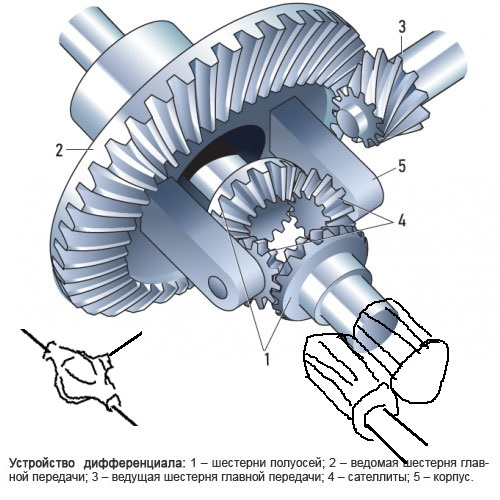
\includegraphics{../ustroistvo-differenciala.jpg}

Выше были изложены пространные теоретические рассуждения, почему мы будем делать именно так. Дальше будет непосредственно описано, как мы это будем делать.

\section{Перейдем к моделированию электрических компонентов:}

\subsection{Источник напряжения}
можно моделировать как вал, вращающийся с постоянной скоростью (который ну ни как невозможно остановить), и подключенный к разностному входу дифференциала. С двух других его концов можно снимать напряжение (они крутятся друг относительно друга с постоянной скоростью).

\subsection{Источник тока}
-- тоже самое, но только используется вал, выдающий постоянный крутящий момент.
Такой вал без нагрузки будет разгонятся до бесконечно большой скорости вращения.

\subsection{Резистор я бы замоделировал так:}
от дифференциала идут лопасти и опускаются в стакан с жидкостью

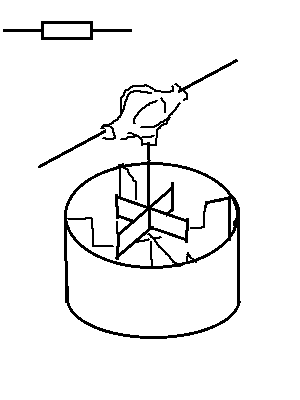
\includegraphics{../R.png}

\begin{itemize}
\item $U=RI$
\item $v=1/\mu F$
\end{itemize}

Чем более вязкая жидкость - тем больше проводимость, тем меньше сопротивление.
Между несоединенными валами трение =0, а сопротивление бесконечное.
А у резистора, у которого заклинило лопасти трение бесконечно большое, а сопротивление нулевое. 
Можно пофантазировать о напряжении пробоя, и трении между валом и его держателями, но по моему это сходство как-то не очень.

\subsection{Конденсатор - маховик, присоединенный к дифференциалу}

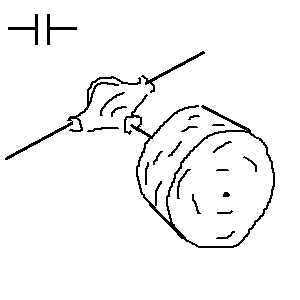
\includegraphics{../C.png}

\begin{itemize}
\item $I=\dot Q; \qquad Q=CU$
\item $F=\dot p; \qquad p=mv$
\end{itemize}

Так же как и в идеальном конденсаторе нет тока утечки, так же и в его модели совсем нет трения.
Так же как сила тока заряжает конденсатор, так же момент сил между валами разгоняет маховик.
В таком конденсаторе на одной пластине всегда заряд $+Q$, а на другой -- $-Q$.

Также емкостью может обладать одиночная сфера (или проводник другой формы). Если он заряжен зарядом Q, то на его поверхности будет потенциал $\varphi$. Их отношение и будет емкостью этого проводника. Это можно замоделировать маховиком без дифференциала.

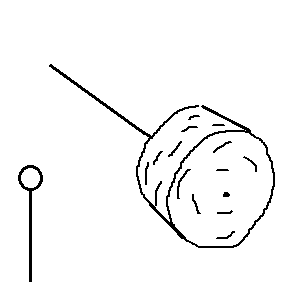
\includegraphics{../C1.png}

\subsection{Катушка - пружинкой, присоединенной к дифференциалу}

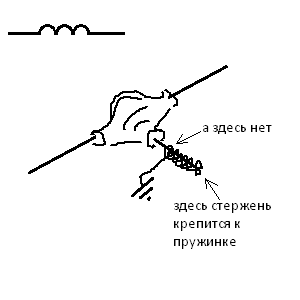
\includegraphics{../L_rot.png}

("Заземлением" будем обозначать неподвижные части конструкции)

\begin{itemize}
\item $U=\dot \Phi; \qquad \Phi=LI$
\item $v=\dot x; \qquad x=(1/k)F$
\end{itemize}

где v - разность скоростей двух валов, а x - относительное смещение.

Если считать, что жесткость пружинки достаточно велика, а момент сил, передаваемый из одного вала в другой, достаточно мал, то катушку можно замоделировать так: 

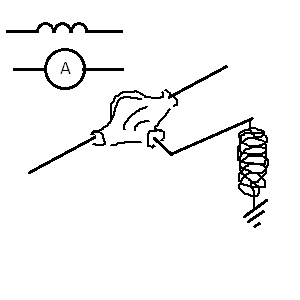
\includegraphics{../L_post.png}

Если пофантазировать, то можно провести аналогию между петлей гистерезиса ферромагнетиков и неупругой деформацией пружинки. Правда в ферромагнетиках нет аналога усталости металла.

А также, модель катушки можно использовать как модель амперметра, если присоединить стрелку к выходу дифференциала.
Ее направление отклонения от положения равновесия будет свидетельствовать о том, в какую сторону вал №1 толкает вал №2. А ее величина - о моменте сил, с которым один вал воздействует на другой, т.е. о силе тока через моделируемую катушку.

И из казалось бы самого простого закона $v=\dot x$ получается, что минус ЭДС катушки = напряжению падения на ней = разности скоростей валов = производной по времени относительного смещения двух валов.
В катушке, которая ни к чему не подключена всегда ток =0, а в ее модели пружина не деформирована.
Но если в катушке есть ток, а потом ее накоротко замкнуть (сверхпроводником), то ток в ней так и останется, 
а ее модель так и будет оставаться в деформированном состоянии.

В принципе в катушке можно обойтись без дифференциала, но в трансформаторе, который содержит в себе пару катушек, так уже не получится.

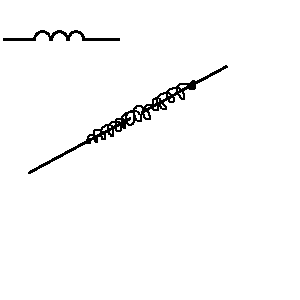
\includegraphics{../L_ndiff.png}

\section{Рассмотрим парочку переходных процессов.}

\subsection{Источник напряжения, ключ, резистор, (изначально незаряженный) конденсатор.}

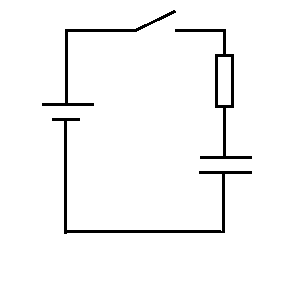
\includegraphics{../RC.png}

Изначально конденсатор не заряжен.
Включаем ключ (после этого $U_C+U_R=U_0$), и на резисторе оказывается напряжение питания, через него начинает течь ток и заряжать конденсатор, что эквивалентно тому, что на конденсаторе начинает расти напряжение, а на резисторе соответственно падать, и ток соответственно тоже начинает падать. Если через некоторое время ключ разомкнуть, то конденсатор так и останется заряженным, а напряжение на резисторе упадет до 0.

Изначально маховик покоится.
Включаем ключ (после этого сумма скоростей маховика и лопастей резистора равна скорости источника напряжения), маховик в начальный момент покоится, а лопасти резистора (невесомые) начинают вращаться, но из-за трения возникает момент сил, который разгоняет маховик. Чем быстрее крутится маховик, тем медленнее крутятся лопасти резистора, и тем с меньшей силой вращают маховик. Если через некоторое время ключ разомкнуть, то маховик продолжит вращаться не меняя своей скорости, а скорость лопастей резистора упадет до 0.

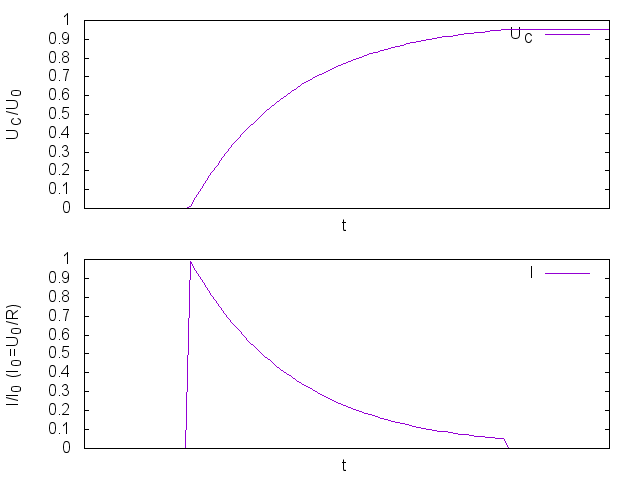
\includegraphics{../plots/RC.png}

\subsection{Источник напряжения, ключ, резистор, катушка.}

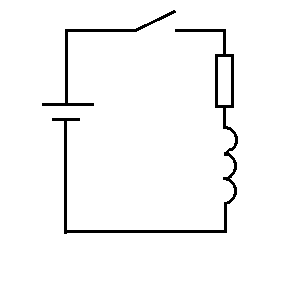
\includegraphics{../RL.png}

Вначале ток равен нулю. Мы включаем ключ (после этого $U_L+U_R=U_0$), и на катушку подается напряжение питания, и оно начинает постепенно разгонять ток через катушку. По мере увеличения тока, увеличивается напряжение падения на резисторе, а значит напряжение, разгоняющее ток в катушке, падает, а значит ток постепенно перестает расти. Если через некоторое время ключ разомкнуть, то в результате практически мгновенной остановки тока на катушке будет очень короткий всплеск ЭДС, полярность которого будет обратна полярности источника напряжения.

Вначале пружинка не растянута. Мы включаем ключ (после этого сумма скоростей деформации пружинки и лопастей резистора равна скорости источника напряжения), и пружинка начинает растягиваться так, как будто в самый начальный момент сопротивление резистора =0. Уже растянутая пружинка начинает оказывать силу на резистор, в результате чего в резисторе возникает разность скоростей, а в пружинке разность скоростей начинает уменьшаться. Чем больше пружинка натянута, тем большую силу она оказывает на резистор, тем больше разность скоростей в резисторе, и тем меньше разность скоростей в катушке (вернее в ее модели), и тем медленнее растягивается пружинка катушки дальше. Если через некоторое время ключ разомкнуть, то в результате практически мгновенного падения нагрузки на пружинку, она очень быстро сожмется в исходное положение.

Механическую модель можно упростить, представив себе покоящуюся на воде невесомую лодку, к которой прикреплена пружинка, а другой конец пружинки внезапно начинают тянуть с постоянной скоростью. Вначале лодка покоится. Потом пружинка начинает натягиваться, и чем больше натягивается, тем больше увлекает за собой лодку, и тем меньше разность между скоростями двух концов пружинки. А если пружинку отпустить (масса кораблика и масса пружинки =0), то кораблик тут же остановится, а пружинка тут же сожмется.

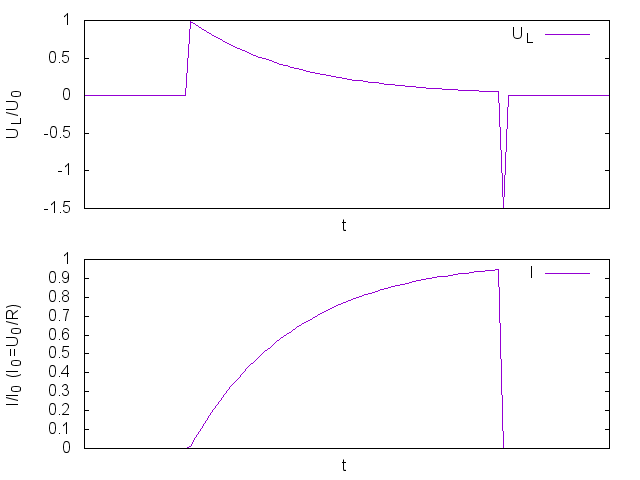
\includegraphics{../plots/RL.png}

\section{И, наконец, механическая модель трансформатора.}

Сам трансформатор описывается также как катушка:

$$U=\dot\Phi; \qquad \Phi=LI$$ где

\begin{itemize}
\item U - столбец напряжений $U_1$ и $U_2$ на 1й и 2й катушках.
\item Ф - столбец магнитных потоков $\Phi_1$ и $\Phi_2$ через 1ю и 2ю катушку.
\item I - столбец токов $I_1$ и $I_2$ через 1ю и 2ю катушку.
\item L - симметричная ($L_{12}=L_{21}$) матрица взаимных индуктивностей $L_{11}, L_{12}, L_{21}, L_{22}$ между соответствующими катушками.
\end{itemize}

Иначе говоря трансформатор описывается системой уравнений:

$$
\begin{cases}
U_1=\dot\Phi_1; \qquad \Phi_1=L_{11}I_1+L_{12}I_2\\
U_2=\dot\Phi_2; \qquad \Phi_2=L_{21}I_1+L_{22}I_2
\end{cases}
\eqno(1)
$$

И чтобы получить механическую модель трансформатора, достаточно взять механические модели двух катушек, и соединить их пружинкой через рычаг:

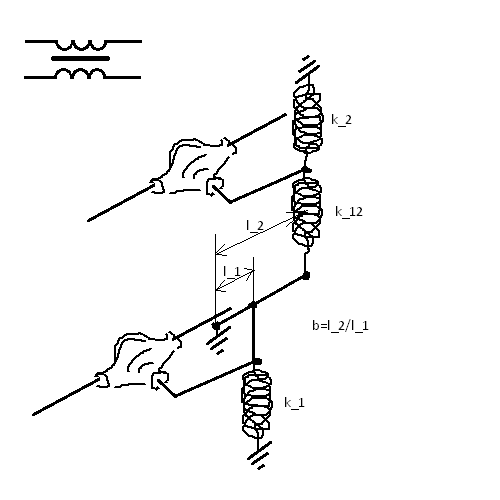
\includegraphics{../T_post.png}

Можно все поступательные пружинки заменить на вращательные, а рычаг заменить на редуктор:

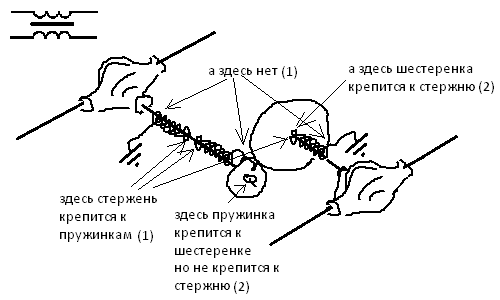
\includegraphics{../T_rot.png}

Найдем уравнения, описывающие эту систему.
Предположим, что верхнее плечо сместилось вверх на $x_1$ (в месте крепления пружины) под действием силы $F_1$, а нижнее сместилось вверх на $x_2$ (в месте крепления пружины) под действием силы $F_2$. Записав вторые законы Ньютона для обоих невесомых плеч, идущих от дифференциалов, получим систему:

$$
\begin{cases}
F_1=k_1 x_1+b k_{12}(bx_1-x_2)\\
F_2=k_2 x_2+k_{12}(x_2-bx_1)
\end{cases}
$$

что тоже самое с

$$
\begin{cases}
F_1=(k_1+b^2k_{12})x_1-bk_{12}x_2\\
F_2=-bk_{12}x_1+(k_2+k_{12})x_2
\end{cases}
$$

ее можно разрешить относительно $x_1$ и $x_2$:

$$
\begin{cases}
v_1=\dot x_1; \qquad x_1=\frac{k_2+k_{12}}{Z} F_1+\frac{bk_{12}}{Z}F_2\\
v_2=\dot x_2; \qquad x_2=\frac{bk_{12}}{Z}F_1+\frac{k_1+b^2k_2}{Z}F_2,
\end{cases}
$$

где $Z=(k_1k_2+k_{12}(k_1+b^2k_2))$

Сравнивая эту систему с (1) получается, что матрицу

$$\begin{pmatrix}
L_{11} & L_{12}\\
L_{21} & L_{22}
\end{pmatrix}$$

следует сопоставлять с матрицей

$$\begin{pmatrix}
k_1+b^2k_{12}	& -bk_{12}	\\
-bk_{12}        &k_2+k_{12}
\end{pmatrix}^{-1}=
\begin{pmatrix}
k_2+k_{12}	& bk_{12}	\\
bk_{12}		& k_1+b^2k_{12}	
\end{pmatrix}
\frac{1}{k_1k_2+k_{12}(k_1+b^2k_2)}
$$

И если у нас есть трансформатор, у которого все витки одинаковые по форме и сечению, на 1й обмотке $N_1$ витков, на второй - $N_2$, и $c$ - доля от магнитного потока, создаваемого 1й катушкой, которая проходит через 2ю катушку (или наоборот - они совпадают) (Если катушки находятся на большом расстоянии, то $c\approx0$ и это фактически две разные катушки. А если катушки близко друг к другу и к тому же соединены сердечником, то $c\approx1$.), то матрица индуктивностей будет выглядеть так:

$$\begin{pmatrix}
L_{11} & L_{12}\\
L_{21} & L_{22}
\end{pmatrix}=\begin{pmatrix}
N_1^2	  & cN_1N_2\\
cN_1N_2 & N_2^2	 
\end{pmatrix}
L_0,
$$

где $L_0$ - коэффициент, зависящий от размеров трансформатора и материала сердечника.

Если в его модели взять $b=N_2/N_1$, то из соотношений

$$L_{11}:L_{12}:L_{22} = N_1^2:cN_1N_2:N_2^2 = k_2+k_{12}:bk_{12}:k_1+b^2k_{12}$$

отношения жесткостей пружин будут выглядеть так:

$$k_1/k_{12} = b^2(1/c-1)$$
$$k_2/k_{12} = 1/c-1$$
$$k_1/k_2 = b^2$$

а матрица индуктивностей модели так:

$$[L] = 
\begin{pmatrix}
(k_2+k_{12})/b^2	& k_{12}/b	\\
k_{12}/b		& k_2+k_{12}	
\end{pmatrix}
\frac{1}{k_2^2+2k_{12}k_2}
$$


т.к. $c \in [0..1]$, то $1/c>1$ => $1/c-1>0$
то соотношения жесткостей тоже >0 (если исключить из модели рычаг, т.е. b=1, то одно из этих соотношений окажется отрицательным, а пружин с отрицательной жесткостью не бывает)
И обратно: при любых соотношения жесткостей пружин

$$k_1/k_{12} =: a_1 >0$$
$$k_2/k_{12} =: a_2 >0$$

и при любом соотношении плеч рычага b>0

$$c=\frac{1}{\sqrt{1+a_1/b^2 +a_2+a_1a_2/b^2}} \in [0..1]$$

$$N_1/(cN_2) = (1+a_2)/b$$
$$N_2/(cN_1) = (1+b^2a_1)/b$$

При $c\to0,$ $k_{12}\to0$ и модели катушек становятся практически независимыми.

При $c\to1,$ $k_{12}\to\infty$ и модели катушек становятся жестко соединены только через рычаг. А индуктивности начинают стремится к

$$[L_{11}]=\frac{k_2+k_{12}}{b^2(k_2^2+2k_{12}k_2)}\to \frac{1}{2b^2k_2}=\frac{1}{2k_1}$$

$$[L]\to
\frac{1}{2}
\begin{pmatrix}
1/k_1	& 1/bk_2\\
1/bk_2	& 1/k_2
\end{pmatrix}
$$

\subsection{Для примера работы трансформатора рассмотрим схему: источник переменного напряжения, трансформатор, резистор}

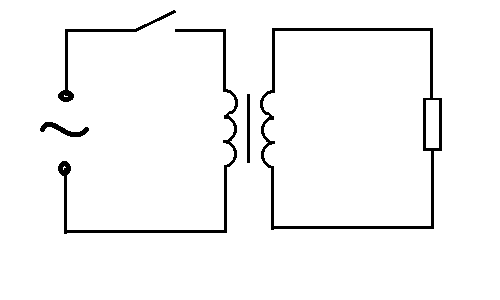
\includegraphics{../TR.png}

и рассчитаем ее

$$
\begin{cases}
U_1=U_0 \cos \omega t\\
U_1=\dot \Phi_1; \qquad \Phi_1=L_{11}I_1+L_{12}I_2\\
U_2=\dot \Phi_2; \qquad \Phi_2=L_{21}I_1+L_{22}I_2\\
U_2+I_2R_2=0
\end{cases}
$$

->

$$
\begin{cases}
U_0 \cos \omega t=L_{11}\dot I_1+L_{12}\dot I_2\\
-I_2R_2=L_{21}\dot I_1+L_{22}\dot I_2
\end{cases}
$$

пусть 

$$\begin{pmatrix}
M_{11}&M_{12}\\
M_{21}&M_{22}
\end{pmatrix}=
\begin{pmatrix}
L_{11}&L_{12}\\
L_{21}&L_{22}
\end{pmatrix}
^{-1}=
\begin{pmatrix}
L_{22}&-L_{21}\\
-L_{12}&L_{11}
\end{pmatrix}
\frac{1}{L_{11}L_{22}-L_{12}^2}=
\begin{pmatrix}
\frac{1}{N_1^2}&-\frac{c}{N_1N_2}\\
-\frac{c}{N_1N_2}&\frac{1}{N_2^2}
\end{pmatrix}\frac{1}{L_0(1-c^2)}
$$

тогда

$$
\begin{cases}
\dot I_1 = M_{11}U_0 \cos \omega t - M_{12}R_2I_2\\
\dot I_2 = M_{21}U_0 \cos \omega t - M_{22}R_2I_2
\end{cases}
$$

последнее уравнение можно переписать в виде

$$\dot I_2 + M_{22}R_2I_2 = M_{21}U_0 \cos \omega t$$

OPOC: $I_2= Ae^{-M_{22}R_2t}$

$$M_{22}=\frac{L_{11}}{L_{11}L_{22}-L_{12}^2} = 
\frac{1}{L_0N_2^2(1-c^2)}>0$$

Этот вклад будет виден только сразу после включения схемы, потом затухнет и не будет участвовать в установившемся режиме трансформации.

Если изменить уравнение так:

$$\dot I_2 + M_{22}R_2I_2 = M_{21}U_0 e^{i \omega t}$$

и искать ЧРНС  в виде $I_2=Be^{i\omega t}$, то придем к алгебраическому уравнению 

$$Bi\omega+M_{22}R_2B=M_{21}U_0$$

=>

$$|B|=\frac{M_{21}U_0}{\sqrt{\omega^2+(M_{22}R_2)^2}}$$

$$tg (-\arg B) = \frac{\omega}{M_{22}R_2}$$

т.к. $Re U_0e^{i\omega t}=U_0 \cos \omega t$, то 

$$I_2=ReBe^{i\omega t}=
\frac{M_{21}U_0}{\sqrt{\omega^2+(M_{22}R_2)^2}}
\cos(\omega t-arctg \frac{\omega}{M_{22}R_2})=$$
$$=\frac{-cU_0}{\sqrt{\omega^2\frac{N_1^2N_2^2}{L_0}(1-c^2)+\frac{N_1^2}{N_2^2}R_2^2}}\cos(\omega t-arctg\frac{\omega N_2^2(1-c^2)L_0}{R_2})\xrightarrow[c\to 1]{}$$
$$\xrightarrow[c\to 1]{} -\frac{N_2}{N_1}\frac{U_0\cos \omega t}{R_2}$$

В случае с механической моделью этой схемы 

$$[I_2]=\frac{-b[U_0]}{\sqrt{\frac{\omega^2}{k_{12}^2}+(\frac{k_2}{k_{12}}+1)^2[R_2]^2}}\cos(\omega t-arctg\frac{\omega}{(k_2+k_{12})[R_2]})\xrightarrow[k_{12}\to \infty]{} \frac{-b[U_0]\cos \omega t}{[R_2]}$$

где величины в квадратных скобках следует заменить их механическими аналогами.

Как и ожидалось, жесткость первой пружинки ни какой роли не играет.

Если упростить механический аналог этой схемы, то у нас получится невесомый кораблик на воде, через пружинку привязанный к берегу, и который через другую пружинку и рычаг двигают туда-сюда по гармоническому закону.

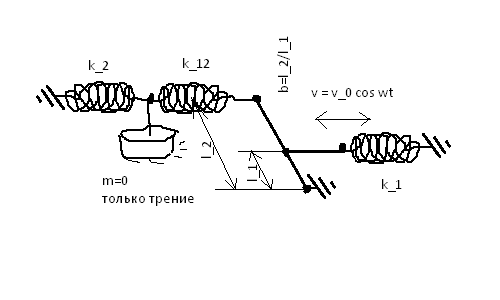
\includegraphics{../T_work.png}

\section{Вместо заключения}
Из нелинейных элементов диод можно храповиком замоделировать, операционный усилитель (который работает так: если напряжение на входе + больше чем напряжение на входе -, то он выдает +U, а если наоборот, то -U) - как на картинке, а транзистор - я не придумал как.

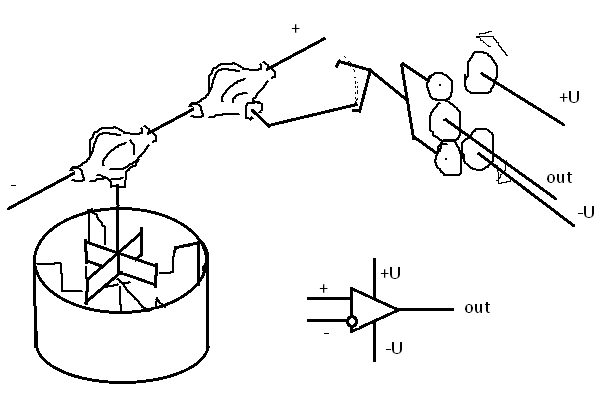
\includegraphics{../OM.png}

В моделях резистора, диода и одиночной катушки можно обойтись без дифференциала. Если пофантазировать, трение валов в креплениях можно интерпретировать как ток утечки через изолятор провода, деформацию валов - как паразитную индуктивность проводов, а момент инерции валов - как паразитную емкость. А вот модели проводов в себе не содержат сопротивления - они сверхпроводящие.

Было бы прикольно, если б кто-нибудь в реальности что-нибудь такое сделал (например из лего-техника, или на 3d принтере напечатал), да на ютуб выложил.

\end{document}
